%%%%%%%%%%%%%%%%%%%%%%%%%%%%%%%%%%%%%%%%%%%%%%%%%%%%%%%%%%%%%%%%%%%%%%%%%%%%%%%%
%2345678901234567890123456789012345678901234567890123456789012345678901234567890
%        1         2         3         4         5         6         7         8

%\documentclass[letterpaper, 10 pt, conference]{ieeeconf}  % Comment this line out if you need a4paper

\documentclass[a4paper, 10pt, conference]{ieeeconf}      % Use this line for a4 paper
\usepackage[brazil]{babel} % coisas em portugues.
\usepackage[T1]{fontenc}
\usepackage{graphicx} % insercao de figuras
% estilo das fontes das lagendas das figuras
\usepackage[font=scriptsize, justification=centering]{caption}
% funcoes matematicas
\usepackage{amsmath} % assumes amsmath package installed
% Define o caminho das figuras
\graphicspath{{imagens/}}

\IEEEoverridecommandlockouts                              % This command is only needed if 
                                                          % you want to use the \thanks command

\overrideIEEEmargins                                      % Needed to meet printer requirements.

% See the \addtolength command later in the file to balance the column lengths
% on the last page of the document

% The following packages can be found on http:\\www.ctan.org
%\usepackage{graphics} % for pdf, bitmapped graphics files
%\usepackage{epsfig} % for postscript graphics files
%\usepackage{mathptmx} % assumes new font selection scheme installed
%\usepackage{times} % assumes new font selection scheme installed
%\usepackage{amssymb}  % assumes amsmath package installed

\title{\LARGE \bf
O Time Carrossel Caipira de Futebol de Robôs
}

% Nomes em ordem alfabetica para facilitar na hora do posicionamento no texto (ideal 5 nomes por linha)
% André N. C. Silva$^{3}$, Danilo W. Nunes$^{1}$, Everton K. Francisco$^{2}$, Marcelo Nuñez$^{1}$, Mário Bordon$^{5}$, Mateus B. Santos$^{1}$, Matheus A. S. Viana$^{3}$, Rafael T. Takagi$^{1}$, Rene Pegoraro$^{4}$, Rodrigo B. R. R. Siqueira$^{1}$, Thiago M. Mochetti$^{3}$
%
\author{{\centering André N. C. Silva$^{3}$, Danilo W. Nunes$^{1}$, Everton K. Francisco$^{2}$, Marcelo Nuñez$^{1}$, Mário Bordon$^{5}$,}%
{\authorblockN \centering Mateus B. Santos$^{1}$, Matheus A. S. Viana$^{3}$, Rafael T. Takagi$^{1}$, Rene Pegoraro$^{4}$, Rodrigo B. R. R. Siqueira$^{1}$,}%
{\authorblockN \centering Thiago M. Mochetti$^{3}$}%
%
\thanks{$^{1}$Danilo W. Nunes (e-mail: danilownunes@gmail.com), Marcelo Nuñez (e-mail: marcelo.nunez@hotmail.com), Mateus B. Santos (e-mail: mateusbatistasantos@gmail.com), Rafael T. Takagi (e-mail: rafaelttakagi@gmail.com) e Rodrigo B. R. R. Siqueira (e-mail: rodrigo.buenorrs@gmail.com) são alunos de Bacharelado em Ciência da Computação.}
\thanks{$^{2}$Everton Kevin Francisco (e-mail: everton\_kelvin@hotmail.com) é aluno de Bacharelado em Sistemas de Informação.}
\thanks{$^{3}$André N. C. Silva (e-mail: neves.andre27@gmail.com), Matheus A. S. Viana (e-mail: mathvna@gmail.com) e Thiago M. Mochetti (e-mail: thiagomochetti@gmail.com) são alunos de Engenharia Elétrica.}
\thanks{$^{4}$Rene Pegoraro (e-mail: pegoraro@fc.unesp.br) é professor do Departamento de Computação.}
\thanks{$^{5}$Mário Bordon (e-mail: mebordon@feb.unesp.br) é professor do Departamento de Engenharia Elétrica.}
}



%%%%%%%%%%%%%%%%%%%%%%%%%%%%%%%%%%%%%%%%%%%%%%%%%%%%%%%%%%%%%%%%%%%%%%%%%%%%%%%%

\begin{document}
\selectlanguage{brazil}


\maketitle
\thispagestyle{empty}
\pagestyle{empty}

% redefinindo abstract como resumo
\renewenvironment{abstract}{\small \bf {\textit{Resumo}---}}

%%%%%%%%%%%%%%%%%%%%%%%%%%%%%%%%%%%%%%%%%%%%%%%%%%%%%%%%%%%%%%%%%%%%%%%%%%%%%%%%

\begin{abstract}
Este artigo apresenta aspectos de hardware e software do time Carrossel Caipira, que representa o Departamento de Computação e o Departamento de Engenharia Elétrica da UNESP, campus de Bauru, na modalidade IEEE Very Small Size de futebol de robôs. O Hardware é composto por três robôs que utilizam Arduino para controle dos motores e recebimento de sinais de rádio, que são enviados por um computador pessoal. O Software, executado neste computador, é composto por um conjunto de módulos que inclui: Visão, Estratégia e Controle.
\end{abstract}

 \section{INTRODU{\c C}ÃO}

O Departamento de Computação da Faculdade de Ciências
da UNESP, campus de Bauru, participa de competições de
futebol de robôs, na modalidade Very Small Size (atualmente
IEEE Very Small), desde 1998, com a realização do 1\textordmasculine
Campeonato Brasileiro de Futebol de Robôs -- CBFR 98. A
pesquisa e o desenvolvimento em futebol de robôs mantém o objetivo de incentivar o uso de
inovações tecnológicas, no campo da robótica, de baixo custo e
com componentes encontrados no mercado nacional. O time de futebol da UNESP
de Bauru é conhecido, desde a primeira edição desta
competição no Brasil, como Carrossel Caipira devido sua
estratégia de jogo. O projeto atual é a sexta versão, de robôs
desenvolvidos para futebol de robôs, com aprimoramentos em
relação ao time de 2017.

No ambiente do futebol de robôs, nesta categoria, os robôs
e a bola são identificados através de uma câmera utilizada
como visão global, posicionada a 2m sobre o campo e alinhada
ao seu centro, que captura imagens da arena. Estas imagens são
processadas digitalmente obtendo as coordenadas dos robôs e da bola.
A partir dessas coordenadas, uma estratégia escolhida e transformada em comandos que são enviados aos
robôs por rádio. Os robôs recebem estes comandos e realizam
as ações correspondentes, modificando a posição dos
elementos presentes no ambiente real, que será capturado
novamente pela câmera. A Fig. \ref{fig:setup_geral} apresenta uma ilustração do
ambiente do futebol de robôs.

% FIGURA
\begin{figure}[!htb]
\centering
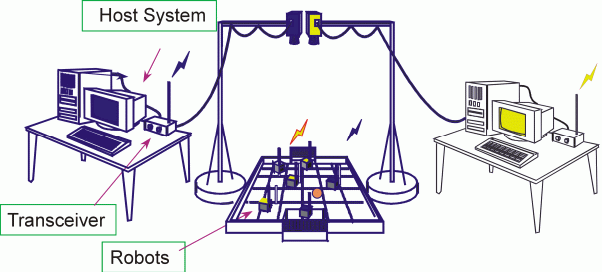
\includegraphics[scale=0.54]{setup_geral1.png}
\caption{Ambiente para futebol de robôs. Fonte:www.mecatronicaatual.com.br/secoes/leitura/950 (2013)}
\label{fig:setup_geral}
\end{figure}
%%%

O futebol robótico abrange diversas áreas do conhecimento.
Na construção do robô são aplicados conceitos de mecânica,
eletrônica e sistemas embarcados. Do ponto de vista do
software, executado no computador pessoal, estão envolvidos
elementos de processamento de imagens, inteligência artificial
e teoria de controle. Essa abrangência faz desta modalidade de
futebol uma ferramenta pedagógica com possíveis aplicações
na graduação.
Esse projeto busca incentivar e facilitar o desenvolvimento
da robótica, para isso o artigo faz uma apresentação das tarefas
realizadas, enfatizando a melhoria aplicada recentemente na arquitetura do software
como um todo e no novo sistema de controle.

\section{SISTEMA DE SOFTWARE DO FUTEBOL DE ROBÔS}

O sistema deste time pode ser representado simplificadamente através do diagrama apresentado na Fig. \ref{fig:esquema_software} que indica as partes principais do processamento. Estas partes são descritas, juntamente com as interações entre elas, na sequência. A CÂMERA captura uma imagem do campo, esta imagem é então processada pelo módulo de VISÃO que determinará as posições atuais dos robôs a partir de suas etiquetas coloridas e a da bola que possui cor alaranjada. A PREVISÃO, com base das informações recebidas do módulo da VISÃO, define as posições mais prováveis que os objetos em campo irão assumir alguns instantes a frente. Com estas posições (presente e futura). O módulo de ESTRATÉGIA calcula os locais do campo que os robôs do time controlado deverão se posicionar. Para realizar estes cálculos, este módulo faz uso de roteiros, que são específicos para cada robô. Basicamente, um roteiro é um conjunto de comportamentos específicos para cara robô que faz com que este assuma uma postura defensiva ou ofenciva durante uma partida. O módulo de CONTROLE, fazendo uso das posição atuais de cada robô (VISÃO) e de seus objetivos (ESTRATÉGIA), determina maior velocidade possível que um robô pode assumir para que este consiga chegar ao seu objetivo e parar, definindo os valores de cada roda a serem enviados aos robôs via rádio, fazendo os robôs se moverem para concluir a estratégia. Todos estes módulos são executados no computador pessoal.

% FIGURA
\begin{figure}[!htb]
  \centering
  % 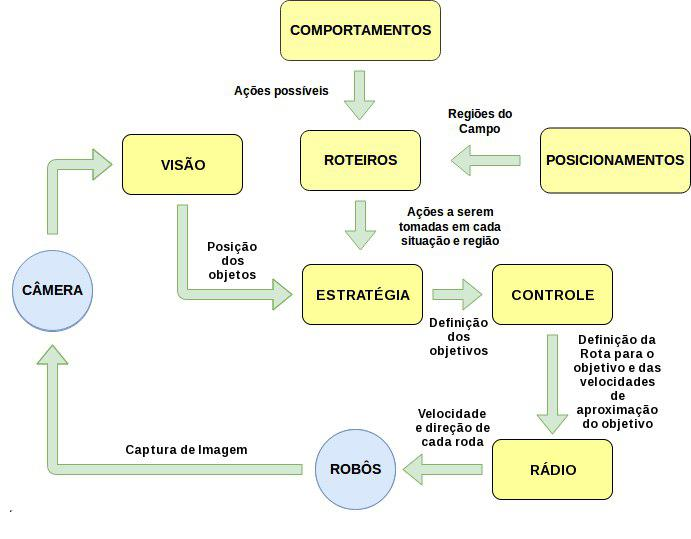
\includegraphics[width=240pt, height=190pt]{esquema_software.jpg}
  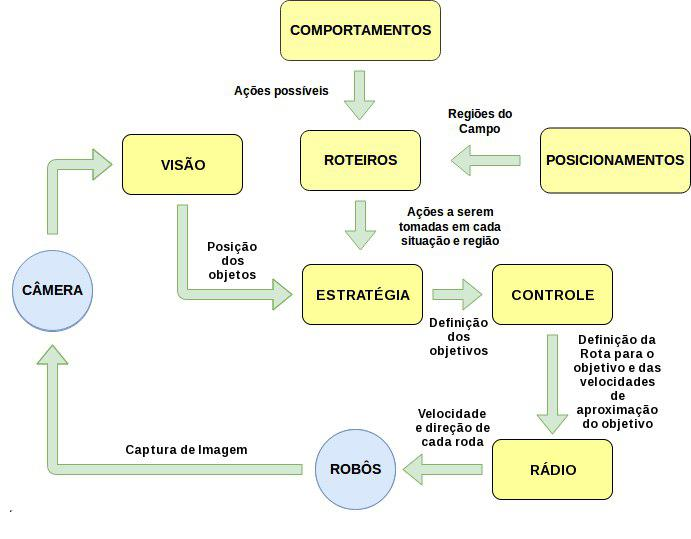
\includegraphics[scale=0.35]{esquema_software.jpg}
  \caption{Diagrama simplificado dos módulos do time Carrossel Caipira.}
  \label{fig:esquema_software}
\end{figure}
%%%

\subsection{Módulo da Visão}

No ambiente de futebol de robôs toda a estratégia e o controle, tanto de baixo nível quanto de alto nível, são baseados na interpretação das imagens captadas pela câmera. Para que isso seja realizado, etiquetas de cores em destaque localizadas no topo dos robôs identificam cada um deles, em relação a seu time e possivelmente sua função, conforme demonstra a Fig. \ref{fig:etiqueta}.

O tempo de execução do ciclo de controle do sistema foi definido pela taxa de aquisição de imagens. Como o time Carrossel Caipira usa câmeras de vídeo convencionais, a taxa é limitada a 30 quadros por segundo. Portanto, a cada período de 33 ms, uma nova imagem refletindo o estado atual do campo torna-se disponível ao computador para processamento. Cada uma dessas imagens é capturada e digitalizada por uma placa
de captura, que disponibiliza, na forma de uma matriz com dimensões 640x480 pixels com três canais (componentes Red, Green, Blue - RGB). Cada um desses pixels deve ser analisado, quanto a sua cor, para identificar se é uma cor de importância ao sistema, esta técnica é chamada de segmentação de cor.

% FIGURA
\begin{figure}[!htb]
\centering
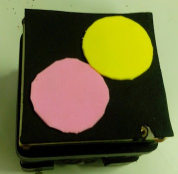
\includegraphics[scale=0.9]{etiqueta.png}
\caption{ Etiqueta de identificação do robô}
\label{fig:etiqueta}
\end{figure}
%%%

\subsection{Módulo de Estratégia}

A estratégia é o módulo responsável por definir a meta de cada robô. Utilizando as coordenadas da bola, dos robôs do time e dos adversários este módulo decide qual é a posição mais indicada para cada robô do time através dos roteiros. Os roteiros são basicamente conjuntos de regras que ditam o comportamento do robô em cada situação. Com as posições pré-determinadas no módulo de posicionamentos e com os comportamentos padronizados no módulo de comportamentos, os roteiros são montados pensando nas situações de jogo. A vantagem deste modelo em relação aos antigos é que através da padronização dos elementos mais básicos da estratégia através destes dois novos módulos é possível montar facilmente montar novos roteiros, o que permite que o time possua diversas posturas às mais diversas situações de jogo, sendo mais ofensivo quando estiver atrás no placar ou mais defensivo quando se deseja tentar manter o resultado, por exemplo.

\subsection{Módulo de Controle}

A partir das coordenadas detectadas pelo módulo de Visão e das coordenadas atribuídas pelos resultados do módulo de Estratégia, o módulo de Controle deve determinar as melhores trajetórias e comandos a ser enviados aos robôs. O cálculo de uma trajetória deve levar em conta o desvio de obstáculos, evitando os outros robôs na arena. Este cálculo é necessário para levar o robô da sua posição atual até a determinada pela estratégia. No caso do time Carrossel Caipira, é empregado um método chamado de campo potencial. Os campos potenciais partem da ideia de forças imaginárias atuando sobre o robô, ideia proposta por Khatib [4], na qual a ''força causada'' pelos obstáculos é de caráter repulsivo e pela meta, de caráter atrativo. Porém a interferência das ''forças'' geradas a partir de vários obstáculos podem produzir locais
ótimos que atrapalham o desempenho do sistema para encontrar um caminho até a meta para o robô.

Para evitar esta situação, Connoly et al. [5] solucionaram o problema utilizando funções harmônicas para o cálculo do campo potencial de ambientes nos quais as posições das paredes, objetos e metas sejam conhecidas, que é o caso do ambiente de futebol de robôs. As funções harmônicas utilizadas são soluções para a equação de Laplace (1).
%
\begin{equation}
\nabla = 0 \ para \ P : R \rightarrow R .
\end{equation}

Assim é definido um Problema de Valor de Contorno na região de atuação do robô utilizando a condição de Dirichlet%
%
\footnote{A condição de contorno de Dirichlet (ou de primeiro tipo) é um tipo de condição de contorno, nomeada em homenagem a Johann Peter Gustav Lejeune Dirichlet (1805-1859). Quando aplicada sobre uma equação diferencial ordinária ou parcial, especifica os valores que uma solução necessita para tomar-se sobre o contorno do domínio}
%
com potencial alto para obstáculos e potencial baixo para a meta. Então, são extraídas as linhas de força, com base no gradiente descendente [5][6] do potencial, que direcionam o robô para sua meta, desviando-o de obstáculos.

Uma vez obtido o campo potencial, tem-se o ângulo ideal que o robô deve atingir para se deslocar até a meta, que chamamos de ângulo objetivo, basta agora calcular a direção e velocidade de cada motor.

\subsection{Interface}

Para comportar toda essas mudanças feitas em diversos módulos da equipe foi também desenvolvida uma nova interface, tendo em mente praticidade e as necessidades de comportar novas funcionalidades. A nova interface foi feita utilizando abas para as principais seções, entre a principal, configurações, outros e ajuda, como pode ser observado na Fig. \ref{fig:interface}.

Na aba principal o foco foi deixar de fácil acesso as funções indispensáveis durante o jogo, entre uma tela para mostrar o q está sendo captado pela câmera, uma tabela para logs e botões para iniciar o software além de situação em que o jogo está, como jogo normal, disputa de bola, w.o., entre outros.

Na aba de configurações se encontram as principais configurações indispensáveis para setup do software, entre escolha dos roteiros, calibração da visão entre outras.

Na aba outros, foram colocadas configurações que geralmente não são usadas, porém podem vir a ser necessárias em situações inesperadas, entre uma opção para gravação em buffer de alguns frames de jogo, uma opção para capturar uma imagem do campo vazio, entre outras.

Finalmente a aba ajuda tem por finalidade explicar as mais diversas funcionalidades do programa, através de uma estrutura separada em seções, pessoas que não conhecem o software podem aprender sobre como utilizá-lo.

% FIGURA
\begin{figure}[!htb]
\centering
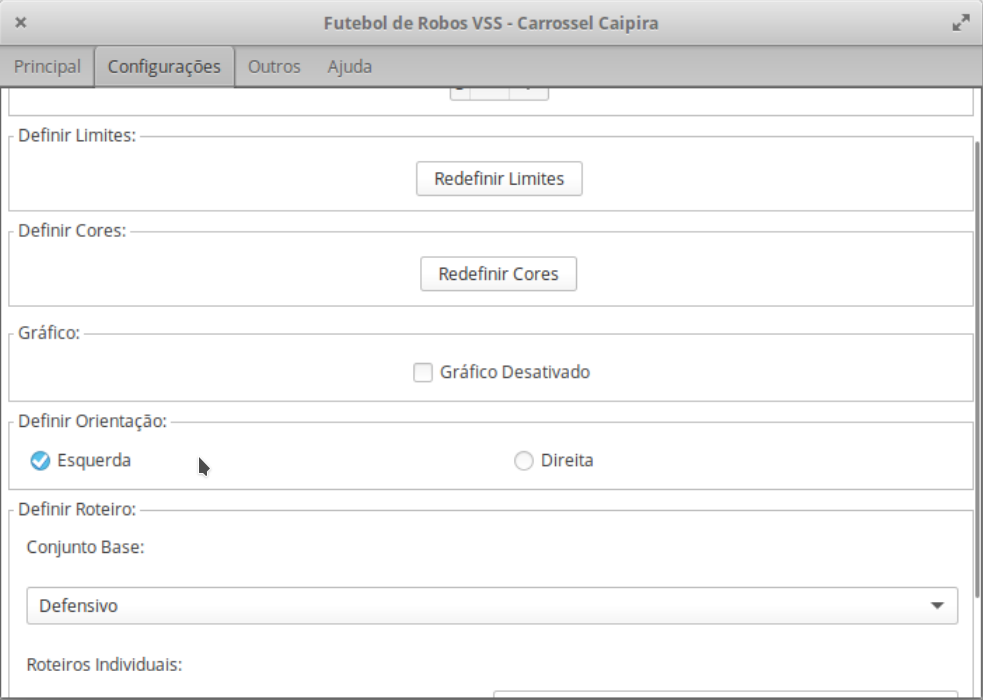
\includegraphics[scale=0.3]{interface.png}
\caption{Nova interface na aba de configurações.}
\label{fig:interface}
\end{figure}
%%%

%
\section{SIMULADOR E TESTES}

O desenvolvimento e os testes utilizaram o simulador no
time da UNESP-Bauru previamente existente. O simulador
executa o módulo de estratégia e o de controle, oriundos do
software executado para o ambiente real, sem alterações nos
códigos. Apenas os arquivos de códigos dos dois módulos
(estratégia e controle) da pasta de fontes destinado ao ambiente
real precisam ser transportados para a pasta do simulador,
nenhuma outra alteração precisa ser realizada. Apesar da
dinâmica ser pouco considerada neste simulador, ele simplifica
a realização de testes dos algoritmos em desenvolvimento, sem
a necessidade da montagem do ambiente real. Uma imagem do
simulador em uma situação de jogo pode ser na vista na Fig. 5.
O simulador pode também apresentar o campo potencial
gerado pelo módulo de controle, Fig. 6.

% FIGURA 5
\begin{figure}[!htb]
\centering
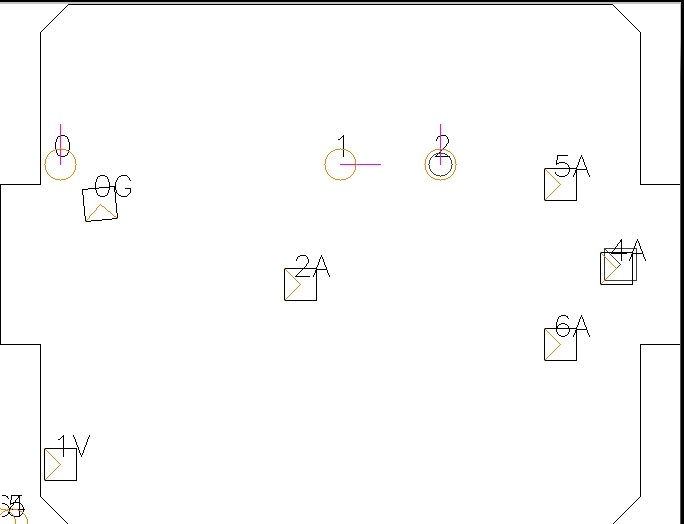
\includegraphics[scale=0.4]{simulador.png}
\caption{Situação representada pelo simulador.}
\label{Rotulo}
\end{figure}
%%%

% FIGURA 6
\begin{figure}[!htb]
\centering
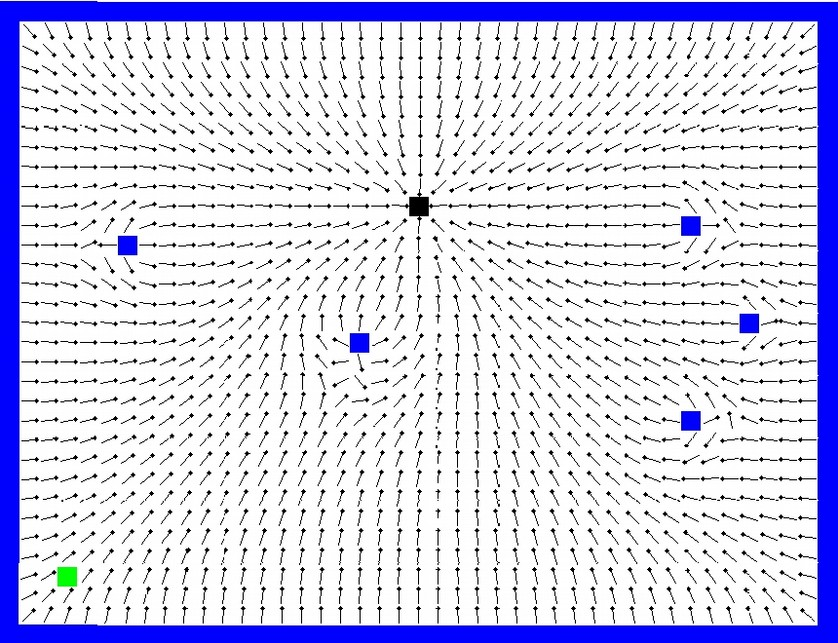
\includegraphics[scale=0.3]{simulador_CP.png}
\caption{Representação do campo potencial para a situação apresentada na
Fig. 5 considerando o robô 1V (volante). Nos quais os quadrados preto, verde
e azul representam respectivamente meta, robô e obstáculo.}
\label{Rotulo}
\end{figure}
%%%

Para que os teste pudessem gerar análises convincentes em
relação ao desenvolvimento da estratégia e do controle, foi
necessário acrescentar uma nova funcionalidade que
permitisse dois times jogarem entre si. Para isso foi
desenvolvido no código do simulador a possibilidade de se
comunicar em rede, de tal forma que houvessem dois times
clientes, cada um com sua estratégia e controle, se
comunicando com o servidor do simulador, que efetiva os
comandos enviados por cada cliente, realizando a
movimentação dos robôs e da bola virtualmente, e fazendo o
papel da visão ao fornecer o estado de cada robô para os times
clientes. Para a comunicação entre os clientes e o servidor
optou-se por um protocolo de comunicação simples, o User
Datagram Protocol (UDP).

Desta forma mudou-se a forma como o simulador funciona.
Na Fig. 7 é apresentado o esquema, de forma simplificada, do
simulador antigo, em que a estratégia recebe o estado do robô,
calcula o objetivo e envia para o controle. O controle vai
calcular a trajetória e o comando que será enviado para cada
roda, que será enviado para o simulador que efetua a
movimentação.

% FIGURA 7
\begin{figure}[!htb]
\centering
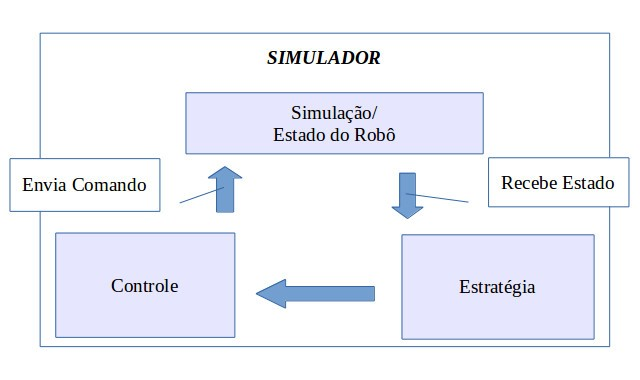
\includegraphics[scale=0.5]{esquema_simulador.png}
\caption{Simulador antes das alterações.}
\label{Rotulo}
\end{figure}
%%%

Na Fig. 8 é apresentado o esquema do simulador atual, no
qual o simulador torna-se um servidor, que recebe os
comandos de cada roda, efetua-os e em seguida envia o estado
do robô para os clientes. Os clientes recebem o estado,
calculam o objetivo através da estratégia e os comandos a ser
enviados para o simulador através do controle, na sequência
esse comando é enviado para o servidor que efetuará a
movimentação dos robôs. Além disso, tem-se a representação
para a conexão de um cliente, mas a representação é a mesma
para dois clientes, que é o caso do futebol de robôs.

% FIGURA 8
\begin{figure}[!htb]
\centering
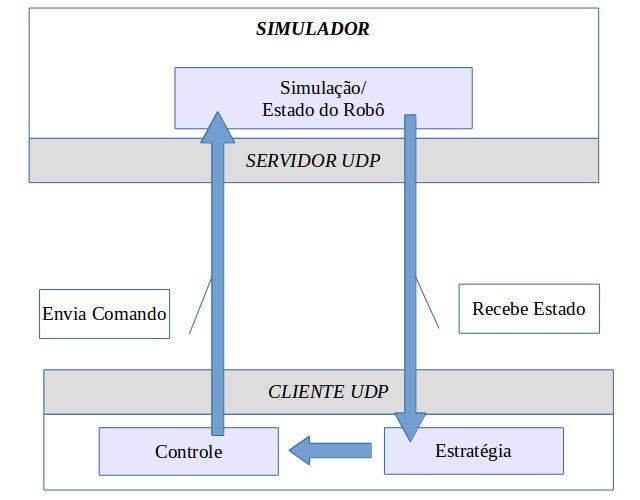
\includegraphics[scale=0.5]{esqumatica_simulador.png}
\caption{ Simulador após alterações, representando uma conexão.}
\label{Rotulo}
\end{figure}
%%%

Assim, o novo simulador permite interação entre dois times
virtuais, levando em consideração a dinâmica, cinemática e
demais constantes físicas referentes ao robô do time Carrossel
Caipira, possibilitando a comparação através de estatísticas
que podem ser coletadas durante a execução do programa, na
figura 9 temos a imagem do novo simulador.

% FIGURA 9
\begin{figure}[!htb]
\centering
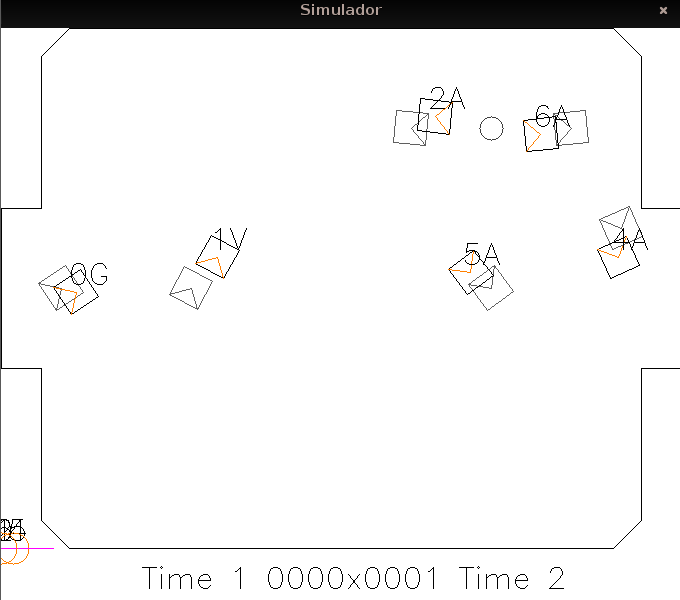
\includegraphics[scale=0.48]{simulador2.png}
\caption{ Simulador após alterações, representando uma conexão.}
\label{Rotulo}
\end{figure}
%%%

Nesta versão, o simulador procura entender o
comportamento da estratégia e controle estudados, através de
situações de jogo como: placar total, gols contra, pênaltis
usufruído pelo time Carrossel Caipira para o desenvolvimento
das pesquisas envolvendo futebol de cometidos, pênaltis
convertidos, gols de cada robô, número de free balls e tempo de
jogo. Além disto, é possível verificar a evolução do placar no
decorrer da simulação e avaliar o intervalo de confiança para
estimar a margem de erro dos dados levantados. A análise
quantitativa dos dados estimula a análise com dados reais feita
no ambiente controlado do laboratório que complementa o
ambiente instrumental robôs. 

%\section{PREVIS{\~A}O DE POSI{\c C}{\~A}O}

Para possibilitar futuramente a realiza{\c c}{\~a}o de passes e
aumentar a acur{\'a}cia dos jogadores com rela{\c c}{\~a}o a bola, est{\'a} foi
desenvolvido um sistema de previs{\~a}o de posi{\c c}{\~a}o da bola e dos demais 
componentes em campo com base no simulador do time Carrossel Caipira.
Como as informa{\c c}{\~o}es do m{\'o}dulo de previs{\~a}o ser{\~a}o usadas pelo
módulo da estratégia, a previs{\~a}o deve ocorrer antes da defini{\c c}{\~a}o do pr{\'o}ximo objetivo. 
Sendo assim, este m{\'o}dulo foi inserido entre o módulo de visão e de estratégia.

Em uma partida existem dois momentos, o de previsão e o de jogo. Enquanto o sistema
está em jogo, todos os m{\'o}dulos trabalham para que cada jogador exer{\c c}a sua fun{\c c}{\~a}o. J{\'a} no
estado de previs{\~a}o, suas fun{\c c}{\~o}es ficam restritas a simular o comportamento de todos os
componentes em campo por um determinado espaço de tempo, porém sem que haja o acionamento dos robôs.

Durante a previs{\~a}o, o m{\'o}dulo de estrat{\'e}gia {\'e} executado utilizando as posi{\c c}{\~o}es 
atuais dos rob{\^o}s e atualiz{\'a}-las com base em seus respectivos roteiros. Atualmente {\'e} feita uma
previs{\~a}o de 30 itera{\c c}{\~o}es, o que corresponde a 1 segundo, que é o suficiente para melhorar o 
desempenho e continuar tendo um previsão realista.   

%% LyX 2.3.0 created this file.  For more info, see http://www.lyx.org/.
%% Do not edit unless you really know what you are doing.
%\documentclass{article}
%\usepackage[utf8]{inputenc}
%\usepackage{graphicx}
%\begin{document}

\section{O HARDWARE DO ROBÔ}
Tendo em vista as propostas para hardware na versão anterior do Robô, para este ano o setor de hardware teve como objetivo a manutenção e atualização dos módulos propostos no ano passado para que ocorra um funcionamento estável, evitando assim mal contato, curtos e possíveis interferências. Ainda tendo em vista a modularidade e praticidade de manutenção do projeto, o robô continuou sendo divido em três módulos (motores, bateria, e placa de circuito impresso), com algumas alterações e uso de outros componentes.

Placa de Circuito Impresso:
Como objetivo de aprimorar a versão anterior, houve uma revisão da placa de circuito impresso dos robôs, tendo em vista otimizar o espaço e a possível utilização de outros componentes como forma de atualização e melhorias no desempenho do robô.

% FIGURA
\begin{figure}[!htb]
    \centering 
        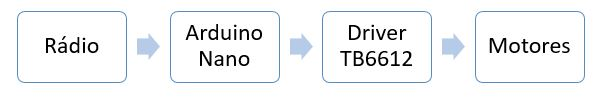
\includegraphics[scale=0.5]{esquema_robo.JPG}
        \caption{Esquema de funcionamento do robô.}
    \label{fig:esquema_robo} 
\end{figure}

Seguindo o diagrama representado na Fig. \ref{fig:esquema_robo}, os componentes do robô são: um módulo de rádio, NRF24l01, um Arduino Nano, um \textit{Driver} para motores, TB6612FNG, e micro motores DC com redução de 50:1. O funcionamento do robô se baseia na transmissão das velocidades através do rádio. Estas informações são transmitidas e armazenadas em um vetor, onde cada par de posições possui a informação de velocidade e sentido que os robôs deverão seguir. O Arduino presente em cada robô recebe as informações via rádio, e envia o equivalente em sinais de PWM para a ponte H, que aciona os motores. A Fig. \ref{fig:Exemplo do vetor de transmissão} exemplifica um vetor onde são armazenadas as informações de velocidade de cada roda de cada robô.

%Figura do funcionamento do rádio
\begin{figure}[!htb]
    \centering 
        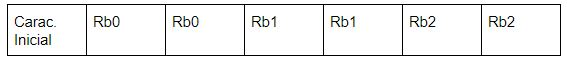
\includegraphics[scale=0.5]{vetor_radio.JPG}
        \caption{Exemplo do vetor de transmissão.}
    \label{fig:Exemplo do vetor de transmissão} 
\end{figure}

%Descrição Componentes
Rádio NRF24L01:
O módulo NRF24L01, ilustrado na Fig. \ref{fig:Radio} opera com frequência em torno de 2.4GHz (faixa de frequência e permite a configuração e construção de um canal de comunicação através da seleção de uma entre 125 frequências (canais) disponíveis, e taxa de transmissão ajustável.

\begin{figure}[!htb]
    \centering
        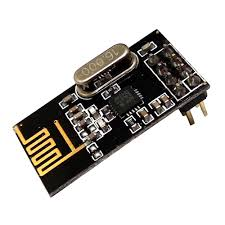
\includegraphics[scale=0.4]{radio.jpg}
        \caption{Módulo de Rádio NRF24L01.}
    \label{fig:Radio} 
\end{figure}

Ponte H (\textit{Driver}) TB6612FNG:
Havendo a necessidade de melhoria no comportamento e controle dos robôs, o \textit{Driver} TB6612FNG, ilustrado na Fig. \ref{fig:TB6612FNG} foi escolhido por melhorar a vida útil do circuito e eliminação de problemas como da força contra eletromotriz e o consumo excessivo, deteriorando precocemente as células de alimentação, impedindo seu pleno funcionamento. Robustez, tamanho reduzido e tecnologia mais atual, essa ponte H possui transistores MOSFETs permitindo atingir frequências de chaveamento em torno de 100KHz, são mais recentes e mais eficientes em relação aos modelos 
com BJTs.

\begin{figure}[!htb]
    \centering 
        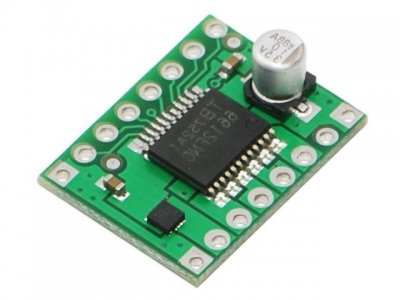
\includegraphics[scale=0.3]{TB6612FNG.jpg}
        \caption{TB6612FNG da Pololu.}
    \label{fig:TB6612FNG} 
\end{figure}

Micromotor DC:
Os motores utilizados são Micromotores DC com redução 50:1 de 6V de tensão nominal, apresentam bom torque. Visto que em versões anteriores já era utilizado e durante algumas simulações se mostrou um ótimo motor, robusto e compacto.

Bateria 18650 (4.2V):
Com grande versatilidade em sua aplicabilidade e facilidade de ser encontrada em dispositivos eletrônicos, a bateria 18650 (Fig. \ref{fig:Célula Li-ion 18650}) é uma excelente opção de alimentação ao VSS devido ao seu tamanho compatível e fidelidade na entrega de energia aos circuitos envolvendo motores com grandes quantidades de picos no consumo.

\begin{figure}[!htb]
    \centering 
        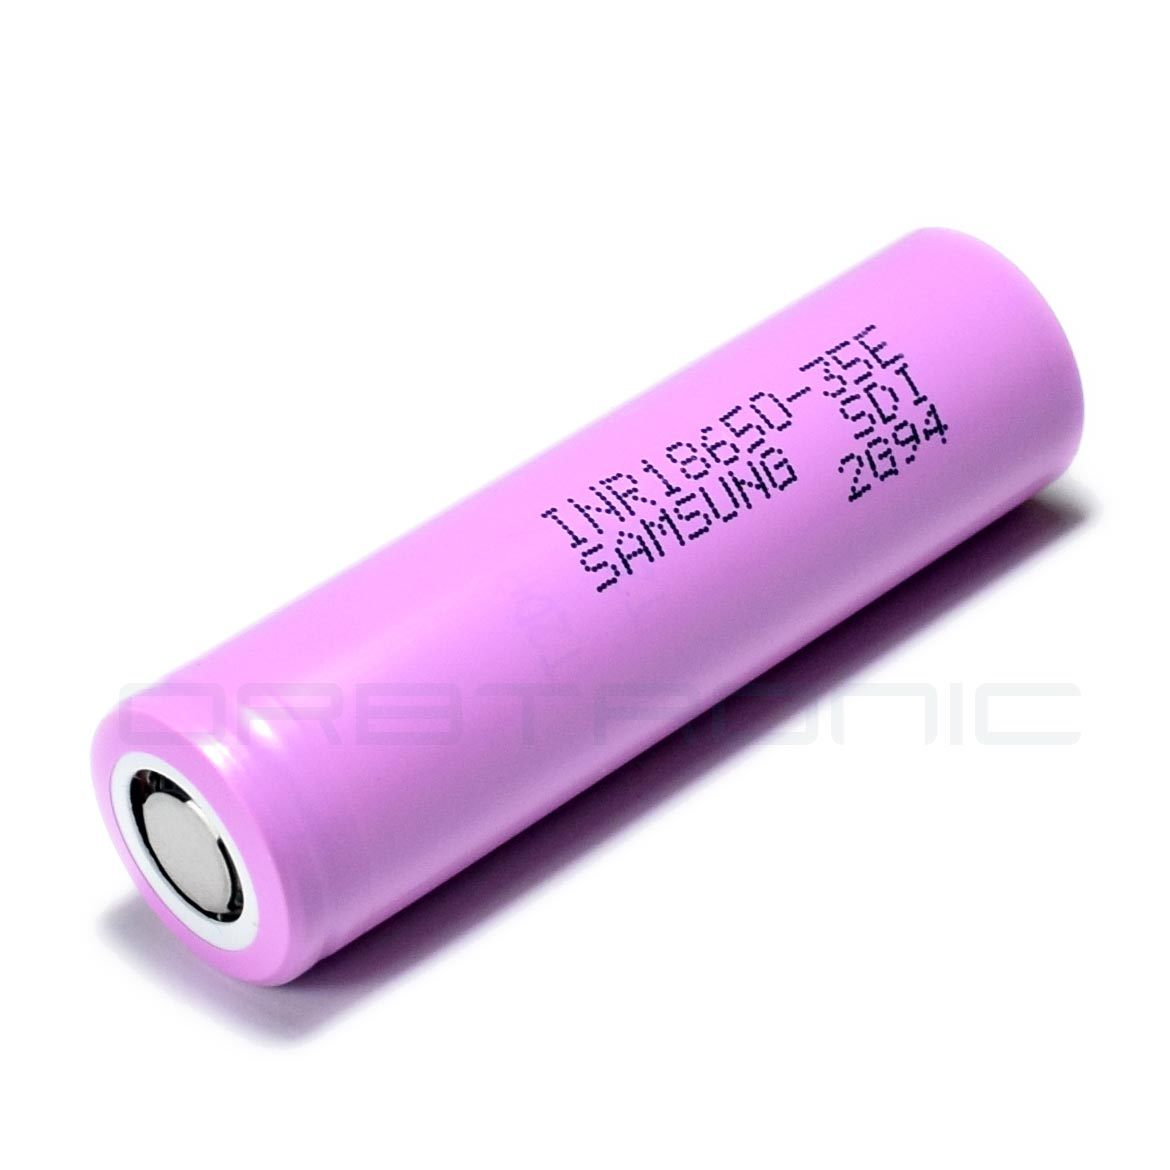
\includegraphics[scale=0.1]{bateria18650.jpg}
        \caption{Célula Li-ion 18650.}
    \label{fig:Célula Li-ion 18650} 
\end{figure}

Apesar de valor relativamente alto, compensa com sua vida útil e espaço que ocupa, se comparado com as células AA com capacidades inferiores e rápida perda no ciclo de vida útil, por conta do perfil que os robôs possuem. 
Seguindo o que foi proposto, além da utilização da bateria de Li-íon 18650, dois componentes eletrônicos foram incluídos no projeto, um módulo TP4056 (Fig. \ref{fig:Módulo Carregador TP4056}), que consiste me um circuito carregador de baterias bem pequeno e compatível com micro-USB, que possibilita uma carga segura e estável das baterias no próprio robô, além de oferecer proteção contra sobrecarga e LEDs que indicam o estado de carga das baterias. 

\begin{figure}[!htb]
    \centering
        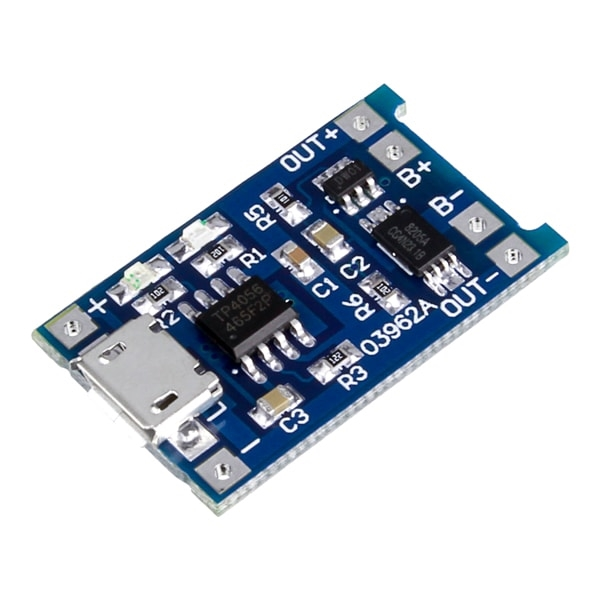
\includegraphics[scale=0.3]{TP4056.jpg}
        \caption{Módulo TP4056.}
    \label{fig:Módulo Carregador TP4056} 
\end{figure}

E um circuito regulador de tensão \textit{Step-Up} MT3608 (Fig. \ref{fig:Regulador de Tensão DC Step-Up MT3608}) também de pequenas dimensões e facilidade no uso,com eficiência de  cerca de 91, grande faixa de operação (2,5 a 28V) e saída de no máximo 2A. A aplicação de ambos no robô foi motivada pela premissa de montar um robô independente de alterações para recarga, estável, e padronizar a tensão de alimentação dos circuitos de controle (Arduino) e dos motores.

\begin{figure}[!htb]
    \centering
        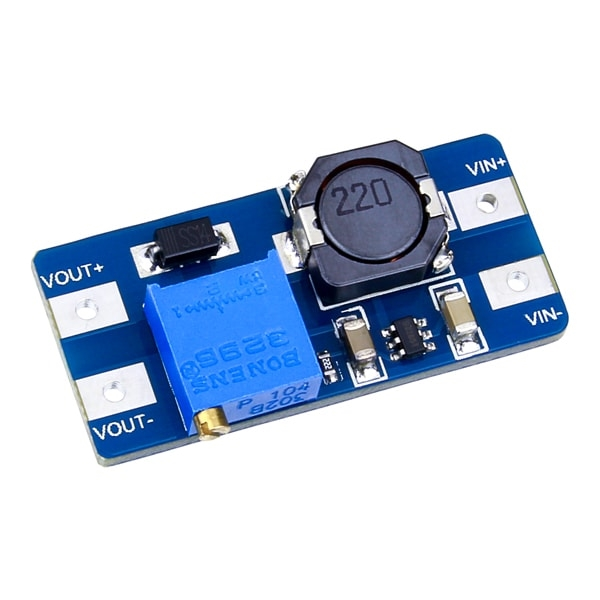
\includegraphics[scale=0.3]{mt3608.jpg}
        \caption{Regulador de Tensão DC Step-Up MT3608.}
    \label{fig:Regulador de Tensão DC Step-Up MT3608} 
\end{figure}

A rotação das rodas, e consequentemente o deslocamento do robô, são determinados por sensores ópticos TCRT5000, que codificam o movimento de dentes reflexivos fixados às rodas em pulsos enviados ao Arduino. Esses pulsos são contados e servem de realimentação ao acionamento direcionado a cada motor, permitindo a aplicação de controle de velocidade aos motores.

Do lado do computador pessoal, o envio dos comandos também ocorre através de um circuito controlado por um Arduino Nano conectado a uma interface USB. Este Arduino recebe os comandos a serem enviados aos robôs e os transmite por meio de um transceptor de rádio NRF24L01 idêntico ao utilizados nos robôs. 
%\end{document}



%%%%%%%%%%%%%%%%%%%%%%%%%%%%%%%%%%%%%%%%%%%%%%%%%%%%%%%%%%%%%%%%%%%%%%%%%%%%%%%%

\begin{thebibliography}{99}

\bibitem{c1} UMBAUGH, S. E.; Digital Image Processing and Analysis: Human and Computer Vision Applications with CVIPtools, Second Edition, CRC Press,November 19, 2010
\bibitem{c2} ALVES, S. F. R.; FERASOLI FILHO, H.; PEGORARO, R.; CALDEIRA, M. A. C.; ROSARIO, J. M.; YONEZAWA, W. M.; Proposal of educational environments with mobile robots; Conference on Robotics, Automation and Mechatronics (RAM), 2011.
\bibitem{c3} COSTA, A. H. R. ; PEGORARO, R. . Construindo robôs autônomos para partidas de futebol: o time GUARANá. Controle \& Automação, Campinas, SP, v. 11, n. 2, p. 141-149, 2000.
\bibitem{c4} KHATIB, O.; Command Dynamic dans l'Espace Opérationnel des Robots Manipulateurs en Présence d'Osbtacles. PhD thesis, Ecole Nationale Supérieure de l'Aéronautique et de l'Espace, Toulouse. em Francês. 1980.
\bibitem{c5} CONNOLLY, C. I., BURNS, J. B.; WEISS, R. Path planning using laplaces equation. In IEEE International Conference on Robotics and Automation, 1990.
\bibitem{c6} CONNOLLY, C. I.; GRUPEN, R. A. On the application of harmonic functions to robotics. Journal of Robotic Systems, 10:931-946, 1993. Placa Arduino Nano 3.0. Dispomível em: <http://arduino.cc/en/Main/ArduinoBoardNano> Acesso em 3 de agosto de 2014.
\bibitem{c7} SANTOS, Rafael, Mecanismo de Previsão de Posição para o Time de Futebol de Robôs da UNESP, Trabalho de Conclusão de Curso do Curso, UNESP - Universidade Estadual Paulista ''Júlio de Mesquita Filho'', Bauru, Brasil, Fev. 2017.

\end{thebibliography} 




\end{document}
